\documentclass[12pt, letterpaper]{article}
\usepackage[utf8]{inputenc}
\usepackage[italian]{babel}
\usepackage[T1]{fontenc}
\usepackage{graphicx}
\graphicspath{}
\usepackage{listings}
\usepackage{svg}

\title{Progetto per il corso di Progetto Automatico di Sistemi Digitali}
\author{Filippo Landi}

\begin{document}
\maketitle

\begin{abstract}
Il mio progetto per il corso di Progetto Automatico di Sistemi Digitali (PASD in breve) consiste nello studio statistico del comportamento di un circuito "multiply and accumulate" (o "mac" in breve) in presenza di alcuni difetti di produzione.
\end{abstract}

\section{Introduzione al progetto}

Il progetto riguarda il collaudo dei sistemi digitali, argomento del corso di PASD.

Al fine di simulare i guasti del circuito userò "HOPE" un simulatore di guasto per circuiti digitali sequenziali sviluppato dall'università VirginiaTech, anche questo proposto durante il corso.  

HOPE legge i circuiti attraverso delle descrizioni della rete (netlist) in formato .bench, quindi il primo punto del progetto sarà studiare la struttura del circuito per implementarlo in questo formato.

Ho deciso di usare Python per aiutarmi con i diversi passaggi del progetto.

Partiamo quindi dalla descrizione del circuito da studiare, passeremo poi alla sua implementazione e in fine ad alcuni studi statistici.

\section{Circuito multiply and accumulate}

Mi è stato richiesto di realizzare un circuito multiply and accumulate (mac) a 8 bit, esso è composto da un moltiplicatore con un sommatore in cascata e un registro per retroazionare le uscite in modo da accumulare i risultati.

Riporto un documento inviatomi dal professore che illustra gli schemi di un circuito di questo tipo a 4 bit.

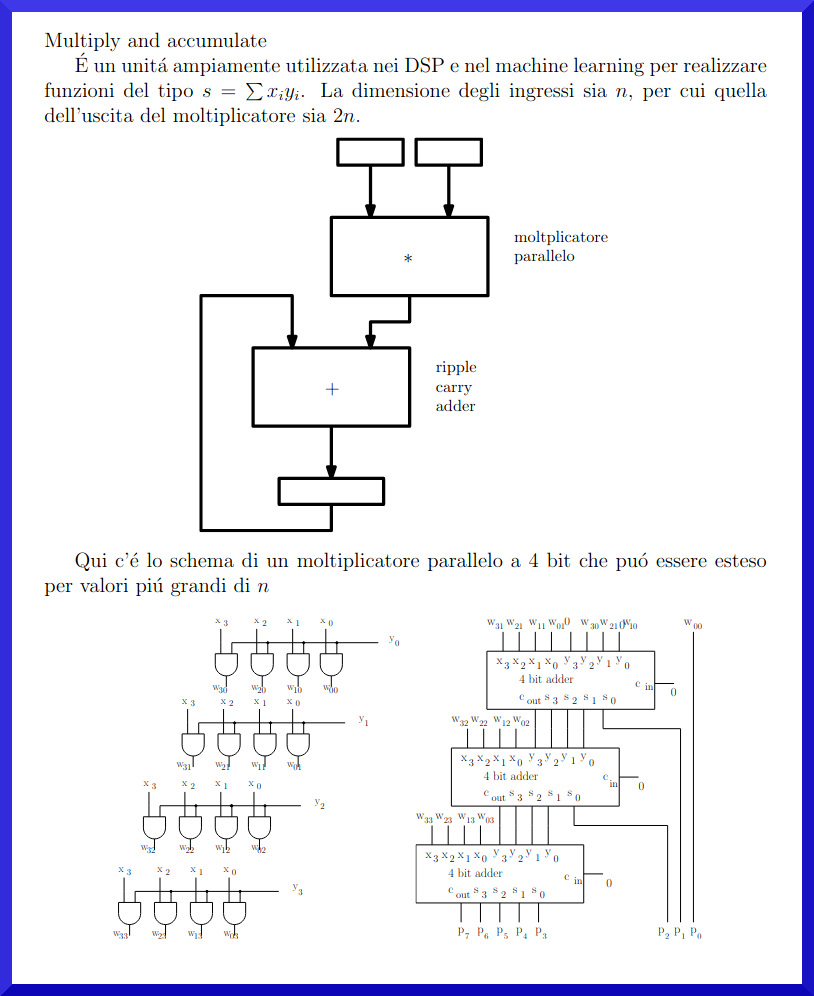
\includegraphics[width=13cm]{mac.png}

\newpage
\subsection{Moltiplicatore}
La struttura del moltiplicatore è ben illustrata nella documentazione:

\begin{itemize}
  \item Ogni segnale X è messo in AND con ogni Y, generando i segnali W.
  \item I segnali W vengono usati da degli adder strutturati su più livelli: si può notare che il numero di livelli è n-1 in quanto al primo livello vengono usati WX1 e WX0, poi i rimanenti WXY nei livelli successivi.
\end{itemize}

\subsection{Sommatore}
È un ripple carry adder con dimensione degli ingressi 2n: un ingresso è dato dall'uscita del moltiplicatore mentre l'altra è data dalle uscite stesse del sommatore retroazionate attraverso dei flip flop tipo D (circuito già integrato in HOPE).

\subsubsection{Ripple Carry Adder}

Usiamo dei ripple carry adder (rca) sia per la cascata di adder del moltiplicatore oltre che per il ripple carry adder successivo con dimensione degli ingressi 2n.

I ripple carry adder nella precedente documentazione erano illustrati a livello register transfer level (RTL) per ovvie ragioni di chiarezza, però per l'implementazione del circuito ci serve vedere come sono fatti a livello di porte logiche.  

I ripple carry adder sono circuiti formati da una serie di adder in cascata:
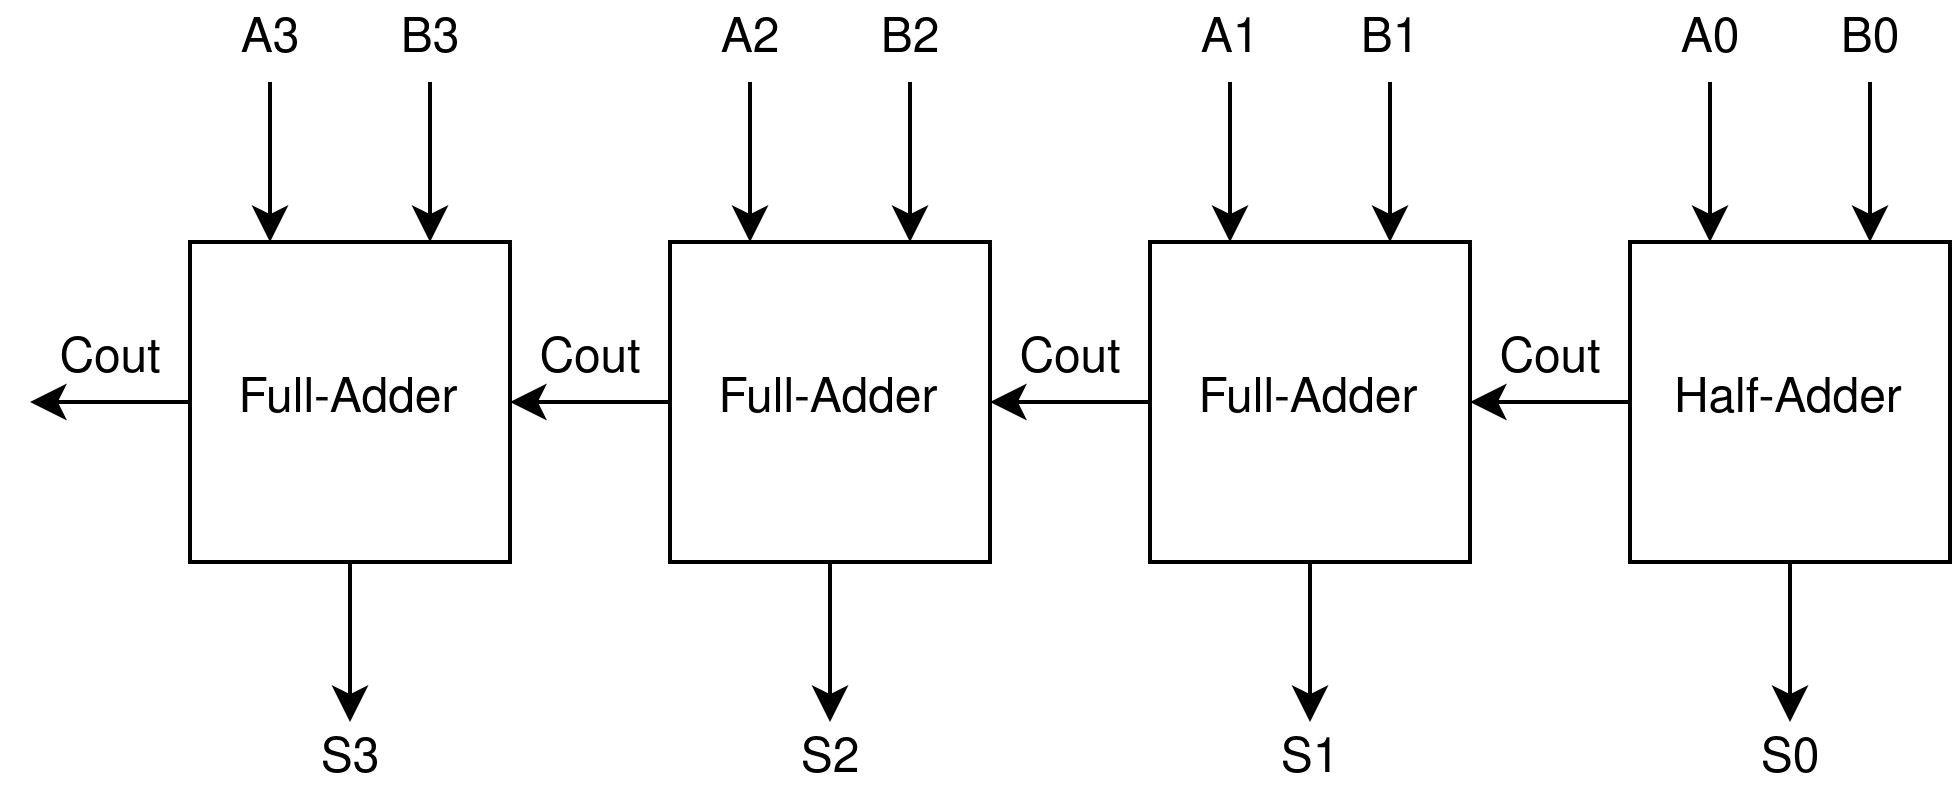
\includegraphics[width=\textwidth]{ripple_carry_adder}

Questo è lo schema che uso del half-adder:
\begin{center}

\includegraphics{half_adder}
\end{center}

Questo è lo schema che uso del full-adder:
\begin{center}
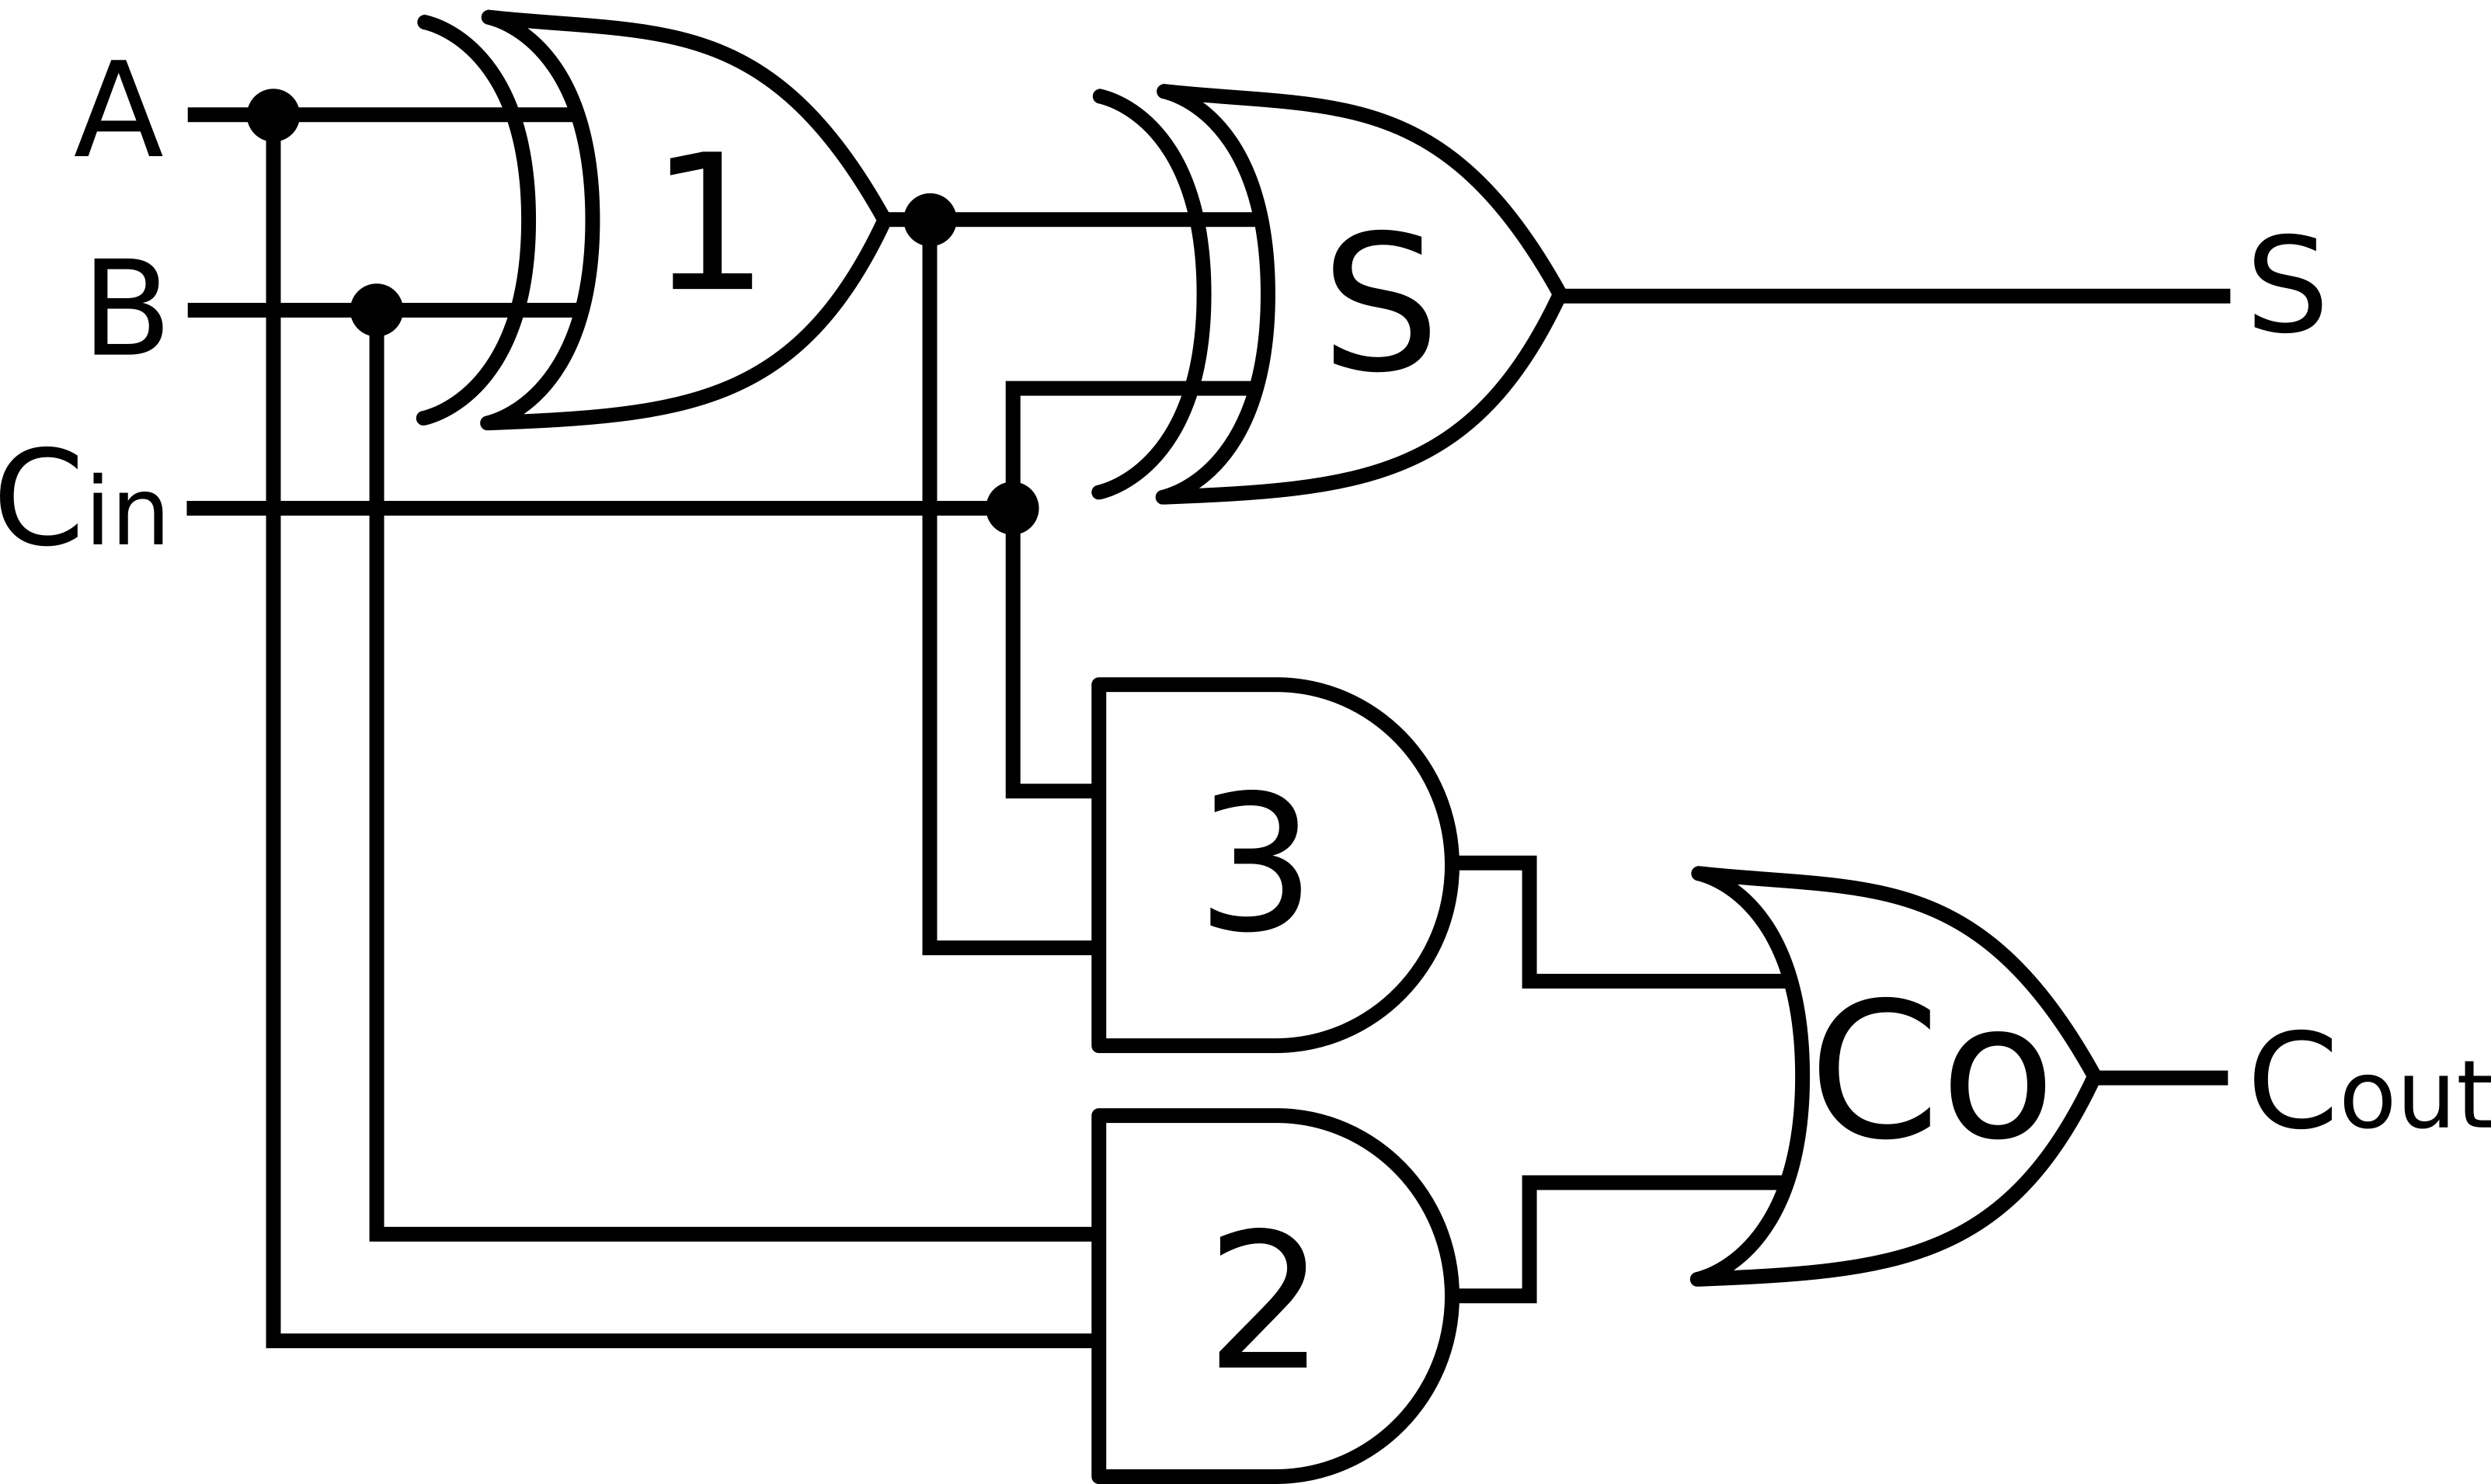
\includegraphics[width=8cm]{full_adder}
\end{center}

Opportunamente collegando le varie porte logiche quindi si ottiene un ripple carry adder.  

\section{Realizzazione del circuito .bench}

La stesura manuale del file .bench del circuito ad 8 bit non mi sembrava un approccio furbo vista l'architettura piuttosto complessa da rappresentare. Probabilmente proseguire con tale metologia avrebbe portato a vari errori: sia banalmente di battitura, sia dovuti alla complessità e quindi errori nel collegamento dei vari segnali. Per questo ho pensato ad una metodologia stile "divide et impera".

In partenza ho scritto alcuni circuiti di prova per esplorare i vari adder e la prima parte del moltiplicatore.
Li trovate nella cartella "circuti\_prova", non sono fondamentali per il progetto però possono aiutare alla comprensione della metodologia usata.

Appurata la struttura dei circuiti base ho creato un singolo file che li mettesse insieme in maniera opportuna (vari cicli for più certe condizioni).
Questo approccio ha portato allo script "mac\_generator.py" che permette di generare il circuito con una dimensione arbitraria degli ingressi da passare come argomento: per generare un mac 4 bit si può scrivere da terminale questo comando Python: "python3 mac\_generator.py 4".  

Il passo successivo sarebbe un approccio più modulare, che otterrebbe lo stesso risultato chiamando sottofunzioni per la varie parti del circuito: per i miei scopi uno script monolitico è più che sufficiente quindi mi fermo con questa versione.

Il codice è ampiamente commentato quindi consiglio di leggerlo per comprenderne il funzionamento.

L'unico punto che potrebbe essere difficoltoso è la comprensione dei vari segnali, proprio per questo un approccio manuale a mio avviso avrebbe portato ad errori di battitura o logici dovuti dalla complessità del circuito.

Descrivo la struttura dei vari segnali sperando di fare un po' di chiarezza:

\begin{itemize}

\item Gli input sono facilmente individuabili e sono X e Y seguiti dal rispettivo peso del bit, es. X0,Y0,X1,Y1 etc.
\item I segnali W ottenuti dagli AND di X e Y sono scritti come "W\_XnYn" (n indica il peso del bit), es. W\_X0Y0.
\item I ripple carry adder contengono half-adder e full-adder:

\begin{itemize}

\item Gli half-adder, come dagli schemi, hanno uscita S e Co (il carry out) e sono usati in generale (con qualche eccezione) per il bit di minor peso (bit 0):
\begin{itemize}
\item Nel moltiplicatore gli rca sono strutturati in livelli:
\begin{itemize}
\item SL0D0 indica l'uscita dell'half-adder al livello (L) 0 del bit di peso (D) 0.
\item CoL0D0 indica il carry out dell'half-adder al livello (L) 0 del bit di peso (D) 0, questo carry out sarà il carry in del full-adder successivo.
\end{itemize}
\item Nel sommatore invece non ci sono più i livelli:
\begin{itemize} 
\item S0 indica l'uscita dell'half-adder per il bit di peso 0.
\item C0 il suo carry out.
\end{itemize}
\end{itemize}

\item I full-adder, come dagli schemi, hanno uscita S e Co con l'aggiunta rispetto gli half-adder dei segnali interni 1,2,3:
\begin{itemize}
\item Nel moltiplicatore gli rca sono strutturati in livelli: 
\begin{itemize}
\item SL0D1 indica l'uscita del full-adder al livello (L) 0 del bit di peso (D) 1
\item lo stesso full-adder avrà CoL0D1, 1L0D1, 2L0D1 e 3L0D1 (carry out e segnali interni).
\end{itemize}
\item Nel sommatore invece non ci sono più i livelli: 
\begin{itemize}
\item S1 indica l'uscita del full-adder per il bit di peso 1
\item Lo stesso full-adder avrà Co1, 11, 21 e 31 (carry out e segnali interni) sempre legati al primo bit.
\end{itemize}
\end{itemize}

\end{itemize}

\end{itemize}

Probabilmente i segnali interni dei full-adder sono i più confusionari, nella mia prima analisi li avevo assegnati numerici e li ho mantenuti così, in caso basta cambiarli con una qualche lettera non assegnata.

Spero che questa spiegazione dei segnali sia esaustiva alla comprensione della struttura del circuito risultante da questo primo script Python.

Gli script originali sono stati scritti con Python 3.8.10 e dovrebbero girare con ogni versione superiore alla 3.6.

Ho anche fatto una conversione per rendere gli script compatibili con Python 2.7, le modifiche non comportano differenze nei file di output.

Se interessa, a livello di sorgenti ci sono state queste modifiche:
\begin{itemize}
\item Python 3.6 aveva introdotto le cosidette "f-strings" molto più comode della metodologia precedente per formattare le stringhe: Python 2.7 ovviamente usa la vecchia formattazione quindi ho dovuto sostituire le f-strings con stringhe formattate con .format().
\item Python 2 suppone che tutti i caratteri siano ascii e quindi se trova lettere accentate da' errore quindi ho forzato l'encoding utf-8 con un "commento magico" nella prima riga di codice.
\item La concatenzione delle stringhe avviene in maniera diversa tra le due versioni per le differenze dovute alla formattazione: con il nuovo metodo le stringhe si concatenano automaticamente, con il vecchio bisogna aggiungere un "+".
\end{itemize}

\section{Testing del circuito con HOPE}

Ottenuto il file .bench contenente la descrizione del circuito possiamo passare ad usare HOPE.

Scrivendo "./hope -h g" si apre la guida utente in cui si possono vedere i vari comandi disponibili.

Useremo un comando HOPE (con alcuni argomenti che spiego in seguito) per i mac 4 bit, 8 bit e 16 bit.
Questo comando ci restituirà un file da analizzare per le statistiche che ci interessano.

\subsection{Analisi del comando HOPE}

Per i vari file useremo il comando: 

\begin{lstlisting}
./hope -F fn -r n -0 -N -s m mac_{bit}.bench
\end{lstlisting}

Dove:
\begin{itemize}
\item fn è il nome di un file da scegliere a piacimento: io aggiungerò il suffisso "\_test" al nome del file bench, ad esempio: mac\_4\_test. 
\item n è il numero di test pattern con cui voler testare il circuito: esploreremo un minimo cosa succede al variare di questo valore.
\item m è un numero per fissare il seme usato da HOPE per la generazione casuale dei vettori: serve per mantenere i test ripetibili, io scelgo di usare il valore 1.
\end{itemize}

Per spiegare meglio il comando riporto una mia traduzione dalla documentazione di HOPE dei vari argomenti:

\begin{itemize}
\item "-F fn": Le uscite del circuito buono e difettoso sono riportate per ogni errore nel file fn. Con questa opzione, l'euristica di fault dropping di HOPE non viene eseguita, vale a dire che tutti i guasti vengono iniettati e simulati in parallelo.(default: l'uscita del circuito difettoso non viene segnalata.) 

NOTA: Le linee dove il guasto viene rivelato hanno un asterisco.

\item "-r n": (Modalità a pattern random)
I pattern di test sono generati in maniera random. La simulazione di guasto termina se se tutti i guasti sono stati rivelato oppure se sono stati applicati n pattern. (default: -r 224)

\item "-0": tutti i flip-flop sono settati inizialmente al livello logico 0

\item "-N": Modalità diagnostica. Il fault dropping non è eseguito. Quindi, tutti i guasti sono simulati per ogni pattern di test. (default: i guasti rivelati durante la simulazione di guasto vengono tolti dalla lista dei guasti.)

\item "-s m": Il seme iniziale del generatore casuale di numeri è impostato da m.
Se m=0, il seme casuale è generato usando l'orario del computer. (default: -s 0)

\end{itemize}

Come spiegato avremo alla fine un file fn da analizzare.

\section{Script getstats.py}

L'analisi del file sarà fatto da uno script python che ho chiamato "gestats.py".

Anche in questo caso il codice è ampiamente commentato e consiglio di leggerlo per comprenderne il funzionamento. 

In breve questo programma esegue questo algoritmo: 
\begin{itemize}
\item Apre il nostro file e con un ciclo lo legge riga per riga
\item Se individua la parola "test" in una riga, vuol dire che sono all'inizio di un nuovo test: da questa riga posso ricavare i vettori di ingresso e l'uscita attuale del circuito.
\item Ad ogni riga successiva ho l'iniezione di un guasto, conto queste righe per sapere il numero di guasti iniettati, inoltre:
\begin{itemize}
\item Una riga con asterisco significa che ho un guasto rivelato in uscita: conto questa riga nel contatore dei guasti rivelati
\item Se non ho un guasto non c'è l'asterisco
\end{itemize}
\item Se individuo di nuovo la parola test:
\begin{itemize}
\item Vuol dire che è terminato il test precedente quindi devo calcolare la statistica che mi interessa che è la probabilità di errore in uscita, data dalla divisione tra i guasti rivelati e i guasti iniettati.
\item Azzero i contatori e continuo.
\end{itemize}
\item Quando esco dal ciclo calcolo le statistiche per l'ultimo test.
\end{itemize}

Per salvare l'output del programma si può ridirigere l'output da terminale a un file a piacimento: es. "getvectors.py mac > output\_mac".
Ridirigere l'output inoltre fa risparmiare molto tempo di esecuzione: mostrare a terminale tutto rallenta di molto l'esecuzione del codice.

Il programma inoltre salva i vari vettori in file di testo sotto forma di array "vectors\_mac", questo è un semplice dump, probabilmente non di grande utilità.

Alla fine di tutto questo lo script che gira su versioni di Python superiori alla 3.6 creerà un grafico a barre utilizzando matplotlib che illustra la probabilità di errore per ogni test.

Purtroppo non sono riuscito a far girare questa feature con Python 2.7, in quanto non sono riuscito ad installare matplotlib per Python 2.7, probabilmente per una questione di ambiente, bisognerebbe provare con degli ambienti virtuali, ma non sono pratico nel loro utilizzo anche se ne comprendo l'utilità.

\section{Analisi dei circuiti mac}

\subsection{Analisi del mac 4 bit}

Incominciamo con l'analisi di un mac a 4 bit.

Creiamo il file .bench con:
\begin{lstlisting}
python3 mac_generator.py 4
\end{lstlisting}
Copiamo il file mac\_4.bench nella cartella di HOPE e lanciamo il comando:
\begin{lstlisting}
./hope -F mac_4_t16 -r 16 -0 -N -s 1 mac_4.bench
\end{lstlisting}
Abbiamo deciso quindi di testare il circuito con un pattern di 16 vettori.
Copiamo il file mac\_4\_t16 nella cartella con i nostri script e lanciamo il comando:
\begin{lstlisting}
python3 getstats.py mac_4_t16
\end{lstlisting}
Questo è il grafico risultate:
\begin{figure}
\centering
\includesvg[width=0.8\columnwidth]{mac_4_t16_stats.svg}
\end{figure}

Ripetendo lo stesso procedimento per con un pattern di 32 vettori di test abbiamo questo grafico:

\begin{figure}
\centering
\includesvg[width=0.8\columnwidth]{mac_4_t32_stats.svg}
\end{figure}

Ripetendo lo stesso procedimento con un pattern di 64 vettori di test abbiamo questo grafico:

\begin{figure}
\centering
\includesvg[width=0.8\columnwidth]{mac_4_t64_stats.svg}
\end{figure}

Si può quindi notare che arrivati dopo un certo numero di test si arriva ad una saturazione.

Vari commenti possibili ed eventuali.

Passiamo al circuito ad 8 bit.

\subsection{Analisi del mac 8 bit}
I vari comandi possono essere estrapolati dai precedenti facilmente.
Usiamo ancora 64 vettori di test.
Il grafico risultante è questo:

\begin{figure}
\centering
\includesvg[width=0.8\columnwidth]{mac_8_t64_stats.svg}
\end{figure}

Abbiamo anche qui un comportamento simile a quello visto prima.

\subsection{Analisi del mac 16 bit}
Vediamo il grafico per il circuito a 16 bit.
\begin{figure}
\centering
\includesvg[width=0.8\columnwidth]{mac_16_t64_stats.svg}
\end{figure}
Vediamo il grafico quando i vettori in questo caso diventano 128.
\begin{figure}
\centering
\includesvg[width=0.8\columnwidth]{mac_16_t128_stats.svg}
\end{figure}


\subsection{Ulteriori analisi}


\end{document}


